\documentclass[border=3pt]{standalone}
% Preâmbulo compartilhado pelos diagramas TikZ da aula 8 de IHR (Métodos de Pesquisa)
\usepackage[T1]{fontenc}
\usepackage[utf8]{inputenc}
\usepackage{lmodern}
\usepackage{amsmath}
\usepackage{xcolor}
\usepackage{tikz}
\usetikzlibrary{arrows.meta,angles,quotes,decorations.pathmorphing,decorations.pathreplacing,calc,
                positioning,shapes.geometric,shapes.misc,backgrounds,fit,
                math}

% Paleta (mesma dos SVGs originais)
% Paleta da disciplina de IHR: acento azul (#1A6FB5), cor de destaque do tema.
% (o nome "dblue" é mantido para não alterar todos os diagramas)
\definecolor{dblue}{HTML}{1A6FB5}
\definecolor{dorange}{HTML}{B3541E}
\definecolor{dgreen}{HTML}{4A7C59}
\definecolor{dred}{HTML}{9C4B4B}
\definecolor{dcream}{HTML}{F4F1EA}
\definecolor{dshade}{HTML}{DDD7C9}

% Função gaussiana (não normalizada por padrão de escala visual)
\pgfmathdeclarefunction{gauss}{3}{%
  \pgfmathparse{1/(#3*sqrt(2*pi))*exp(-((#1-#2)^2)/(2*#3^2))}%
}

% Estilos comuns (prefixo d... para não colidir com chaves internas do pgf)
\tikzset{
  >={Stealth[length=2mm]},
  dguide/.style={gray!55, dashed, line width=0.4pt},
  daxis/.style={gray!60, line width=0.7pt, ->},
  dbody/.style={fill=black!3, draw=black!80, line width=1pt},
  dacc/.style={draw=dblue, line width=1pt},
  dlbl/.style={black!55, font=\small},
  dsub/.style={black!45, font=\footnotesize},
  dstate/.style={circle, draw=black!80, fill=dcream, line width=1pt,
                 minimum size=17mm, font=\large, inner sep=1pt},
  dobs/.style={circle, draw=black!80, fill=dshade, line width=1pt,
               minimum size=14mm, font=\large, inner sep=1pt},
  dbox/.style={rounded corners=2pt, draw=black!80, fill=dcream, line width=1pt,
               align=center, inner sep=6pt},
  dop/.style={circle, draw=black!80, fill=white, line width=1pt,
              minimum size=6mm, inner sep=0pt, font=\small},
  dtrans/.style={->, dblue, line width=1pt},
  dmeas/.style={->, dorange, line width=1pt},
  dcurve/.style={line width=1pt, dblue},
  dcurveb/.style={line width=1.4pt, dorange},
}

\begin{document}
\hyphenpenalty=10000 \exhyphenpenalty=10000 \tolerance=9999 \emergencystretch=3em
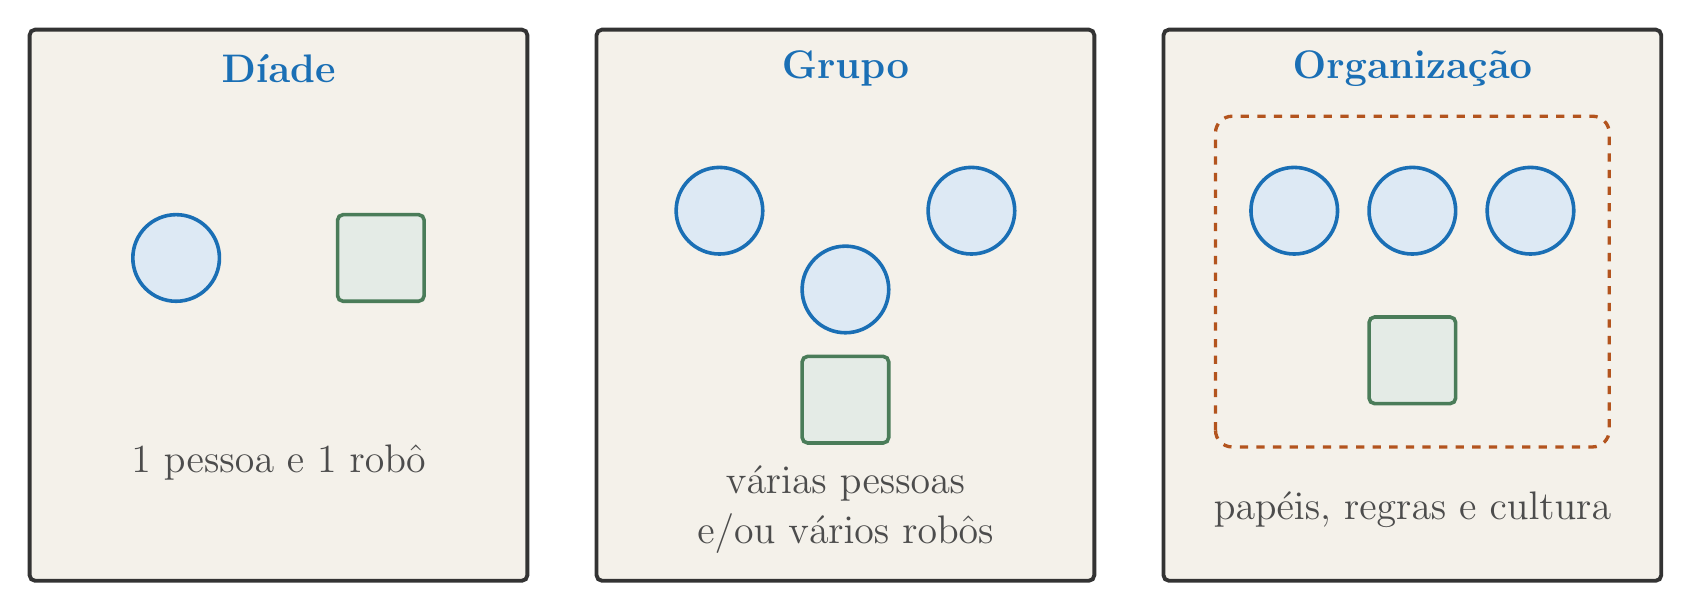
\begin{tikzpicture}[x=1cm,y=1cm]
  \tikzset{pp/.style={circle, draw=dblue, fill=dblue!15!white, line width=1.3pt, minimum size=11mm}}
  \tikzset{rb/.style={rounded corners=2pt, draw=dgreen, fill=dgreen!15!white, line width=1.3pt, minimum size=11mm}}
  \tikzset{pn/.style={dbox, text width=5.9cm, minimum height=7.0cm, line width=1.4pt}}
  \node[pn] at (0,0) {};
  \node[font=\Large\bfseries, dblue] at (0,3.0) {Díade};
  \node[pp] at (-1.3,0.6) {}; \node[rb] at (1.3,0.6) {};
  \node[font=\Large, black!70, align=center, text width=5.3cm] at (0,-2.0) {1 pessoa e 1 robô};
  \node[pn] at (7.2,0) {};
  \node[font=\Large\bfseries, dblue] at (7.2,3.0) {Grupo};
  \node[pp] at (5.6,1.2) {}; \node[pp] at (7.2,0.2) {}; \node[pp] at (8.8,1.2) {};
  \node[rb] at (7.2,-1.2) {};
  \node[font=\Large, black!70, align=center, text width=5.3cm] at (7.2,-2.6) {várias pessoas e/ou vários robôs};
  \node[pn] at (14.4,0) {};
  \node[font=\Large\bfseries, dblue] at (14.4,3.0) {Organização};
  \draw[dorange, dashed, line width=1.2pt, rounded corners=6pt] (11.9,-1.8) rectangle (16.9,2.4);
  \node[pp] at (12.9,1.2) {}; \node[pp] at (14.4,1.2) {}; \node[pp] at (15.9,1.2) {}; \node[rb] at (14.4,-0.7) {};
  \node[font=\Large, black!70, align=center, text width=5.3cm] at (14.4,-2.6) {papéis, regras e cultura};
\end{tikzpicture}
\end{document}
